\documentclass{beamer}
\mode<presentation>
\usepackage{amsmath}
\usepackage{amssymb}
%\usepackage{advdate}
\usepackage{adjustbox}
\usepackage{subcaption}
\usepackage{enumitem}
\usepackage{multicol}
\usepackage{mathtools}
\usepackage{listings}
\usepackage{url}
\def\UrlBreaks{\do\/\do-}
\usetheme{Boadilla}
\usecolortheme{lily}
\setbeamertemplate{footline}
{
	\leavevmode%
	\hbox{%
		\begin{beamercolorbox}[wd=\paperwidth,ht=2.25ex,dp=1ex,right]{author in head/foot}%
			\insertframenumber{} / \inserttotalframenumber\hspace*{2ex} 
	\end{beamercolorbox}}%
	\vskip0pt%
}
\setbeamertemplate{navigation symbols}{}

\providecommand{\nCr}[2]{\,^{#1}C_{#2}} % nCr
\providecommand{\nPr}[2]{\,^{#1}P_{#2}} % nPr
\providecommand{\mbf}{\mathbf}
\providecommand{\pr}[1]{\ensuremath{\Pr\left(#1\right)}}
\providecommand{\qfunc}[1]{\ensuremath{Q\left(#1\right)}}
\providecommand{\sbrak}[1]{\ensuremath{{}\left[#1\right]}}
\providecommand{\lsbrak}[1]{\ensuremath{{}\left[#1\right.}}
\providecommand{\rsbrak}[1]{\ensuremath{{}\left.#1\right]}}
\providecommand{\brak}[1]{\ensuremath{\left(#1\right)}}
\providecommand{\lbrak}[1]{\ensuremath{\left(#1\right.}}
\providecommand{\rbrak}[1]{\ensuremath{\left.#1\right)}}
\providecommand{\cbrak}[1]{\ensuremath{\left\{#1\right\}}}
\providecommand{\lcbrak}[1]{\ensuremath{\left\{#1\right.}}
\providecommand{\rcbrak}[1]{\ensuremath{\left.#1\right\}}}
\theoremstyle{remark}
\newtheorem{rem}{Remark}
\newcommand{\sgn}{\mathop{\mathrm{sgn}}}
\providecommand{\abs}[1]{\left\vert#1\right\vert}
\providecommand{\res}[1]{\Res\displaylimits_{#1}} 
\providecommand{\norm}[1]{\lVert#1\rVert}
\providecommand{\mtx}[1]{\mathbf{#1}}
\providecommand{\mean}[1]{E\left[ #1 \right]}
\providecommand{\fourier}{\overset{\mathcal{F}}{ \rightleftharpoons}}
%\providecommand{\hilbert}{\overset{\mathcal{H}}{ \rightleftharpoons}}
\providecommand{\system}{\overset{\mathcal{H}}{ \longleftrightarrow}}
%\newcommand{\solution}[2]{\textbf{Solution:}{#1}}
%\newcommand{\solution}{\noindent \textbf{Solution: }}
\providecommand{\dec}[2]{\ensuremath{\overset{#1}{\underset{#2}{\gtrless}}}}
\newcommand{\myvec}[1]{\ensuremath{\begin{pmatrix}#1\end{pmatrix}}}
\let\vec\mathbf

\lstset{
	%language=C,
	frame=single, 
	breaklines=true,
	columns=fullflexible
}

\numberwithin{equation}{section}

\title{Matgeo Presentation}
\author{Eshan Sharma \\ EE24BTECH11022}

\date{\today} 
\begin{document}
	
	\begin{frame}
		\titlepage
	\end{frame}
	
	\section*{Outline}
	\begin{frame}
		\tableofcontents
	\end{frame}
	\section{Problem}
	\begin{frame}
		\frametitle{Problem Statement}
		Consider two points $\vec{P}$ and $\vec{Q}$ with position vectors $\overrightarrow{OP} = \overrightarrow{3a} - \overrightarrow{2b}$ and $\overrightarrow{OQ} = \overrightarrow{a} + \overrightarrow{b}$. Find the position vector of a point $\vec{R}$ which divides the line joining $\vec{P}$ and $\vec{Q}$ in the ratio 2 : 1, \\ 
		i) internally, and \\
		ii) externally
	\end{frame}
	
	%\subsection{Literature}
	\section{Solution}
	\subsection{Input parameters}
	\begin{frame}
		\frametitle{Input Parameters}
		\begin{table}[H]    
			\centering
			\begin{tabular}[12pt]{ |c|c|c|}
    \hline
    \textbf{Symbol} & \textbf{Value} & \textbf{Description} \\
    \hline
    \textbf{S} & $3cm$ & length of side of square\\
    \hline
    \end{tabular}

		\end{table}
	\end{frame}
	\subsection{Linear equation}
	\begin{frame}
		\frametitle{Linear Equation}
		For the internal division,
		%\begin{enumerate}[label=(\roman*)]
		\begin{align}
			\overrightarrow{OR} &= \frac{\overrightarrow{OP} + \vec{m} \times \overrightarrow{OQ}}{1+\vec{m}} 
		\end{align}
		%
		For the external division,
		%\begin{enumerate}[label=(\roman*)]
		\begin{align}
			\overrightarrow{OR} &= \frac{\vec{m} \times \overrightarrow{OQ} - \overrightarrow{OP}}{\vec{m} - 1} 
		\end{align}
		%
		where
		\begin{align}
			\vec{m} = 2
		\end{align}
	\end{frame}
	\subsection{Calculations}
	\begin{frame}
		\frametitle{Calculations}
		Internal Division:
		\begin{align}
			\overrightarrow{OR} &= \frac{1 \times \overrightarrow{OP} + 2 \times \overrightarrow{OQ}}{3} \\
			\overrightarrow{OR} &= \frac{1 \times (3\overrightarrow{a} - 2\overrightarrow{b}) + 2 \times (\overrightarrow{a} + \overrightarrow{b})}{3} \\
			\overrightarrow{OR} &= \frac{3\overrightarrow{a} - 2\overrightarrow{b} + 2\overrightarrow{a} + 2\overrightarrow{b}}{3} \\
			\overrightarrow{OR} &= \frac{5\overrightarrow{a}}{3}
		\end{align}
	\end{frame}
	\begin{frame}
		External Division:
		\begin{align}
			\overrightarrow{OR} &= \frac{2 \times \overrightarrow{OQ} - 1 \times \overrightarrow{OP}}{2 - 1} \\
			\overrightarrow{OR} &= \frac{2 \times (\overrightarrow{a} + \overrightarrow{b}) - 1 \times (3\overrightarrow{a} - 2\overrightarrow{b})}{1} \\
			\overrightarrow{OR} &= \frac{2\overrightarrow{a} + 2\overrightarrow{b} - 3\overrightarrow{a} + 2\overrightarrow{b}}{1} \\
			\overrightarrow{OR} &= \overrightarrow{-a} + 4\overrightarrow{b}
		\end{align}
		The codes below verifies the same.
	\end{frame}
	
	\section{C Code}
	\begin{frame}[fragile]
	\frametitle{C Code}
	\begin{lstlisting}[language=C]
#include <stdio.h>
			
int main() {
	FILE *fptr;
	fptr = fopen("division_points.txt", "w");
				
	if (fptr == NULL) {
		printf("Error opening file!\n");
		return 1;
	}
				
	// Position vectors for points P and Q
	float Px = 3.0, Py = -2.0; // Point P (3a - 2b)
	float Qx = 1.0, Qy = 1.0; // Point Q (a + b)
	\end{lstlisting}
	\end{frame}
	\begin{frame}[fragile]
	\begin{lstlisting}[language=C]
	// Internal division ratio m:n (2:1)
	int m_internal = 1, n_internal = 2;
	float Rx_internal = (m_internal * Px + n_internal * Qx) / (m_internal + n_internal);
	float Ry_internal = (m_internal * Py + n_internal * Qy) / (m_internal + n_internal);
	// External division ratio m:n (2:1)
	int m_external = 2, n_external = 1;
	float Rx_external = (m_external * Qx - n_external * Px) / (m_external - n_external);
	float Ry_external = (m_external * Qy - n_external * Py) / (m_external - n_external);
	\end{lstlisting}
	\end{frame}
	\begin{frame}[fragile]
	\begin{lstlisting}[language=C]
	// Save the results to the file
	fprintf(fptr, "%f%f\n", Rx_internal, Ry_internal); // Internal division
	fprintf(fptr, "%f%f\n", Rx_external, Ry_external); // External division
	
	fclose(fptr);
	printf("Division points saved to division_points.txt\n");
	return 0;
	}
	\end{lstlisting}
	\end{frame}

\section{Python Code}
\begin{frame}[fragile]
\frametitle{Python Code for Plotting}
\begin{lstlisting}[language=Python]
import numpy as np
import matplotlib.pyplot as plt

# Load the division points from the text file
points = np.loadtxt("division_points.txt")

# Extracting the internal and external division points
R_internal = points[0]  # Internal division point
R_external = points[1]  # External division point

# Define points P and Q
P = np.array([3, -2])   # Point P
Q = np.array([1, 1])    # Point Q

plt.figure(figsize=(10, 5))
\end{lstlisting}
\end{frame}
\begin{frame}[fragile]
\begin{lstlisting}[language=Python]
# Plotting Internal Division
plt.subplot(1, 2, 1)
plt.plot([P[0], Q[0]], [P[1], Q[1]], 'bo-', label="Line PQ")
plt.plot(R_internal[0], R_internal[1], 'ro', label="Internal Division R")
plt.text(P[0], P[1], 'P', fontsize=12, ha='right')
plt.text(Q[0], Q[1], 'Q', fontsize=12, ha='right')
plt.text(R_internal[0], R_internal[1], 'R', fontsize=12, ha='right')
plt.title('Internal Division of Line Segment')
plt.grid(True)
plt.axhline(0, color='black', linewidth=0.5)
plt.axvline(0, color='black', linewidth=0.5)
plt.legend()
\end{lstlisting}
\end{frame}
\begin{frame}[fragile]
\begin{lstlisting}[language=Python]
# Plotting External Division
plt.subplot(1, 2, 2)
plt.plot([P[0], Q[0]], [P[1], Q[1]], 'bo-', label="Line PQ")
plt.plot(R_external[0], R_external[1], 'ro', label="External Division R")
plt.text(P[0], P[1], 'P', fontsize=12, ha='right')
plt.text(Q[0], Q[1], 'Q', fontsize=12, ha='right')
plt.text(R_external[0], R_external[1], 'R', fontsize=12, ha='right')
plt.title('External Division of Line Segment')
plt.grid(True)
plt.axhline(0, color='black', linewidth=0.5)
plt.axvline(0, color='black', linewidth=0.5)
plt.legend()

plt.tight_layout()
plt.show()

\end{lstlisting}
\end{frame}

\section{Plot of the division}
\begin{frame}
	\frametitle{Plot of the division}
	\begin{figure}[H]
		\centering
		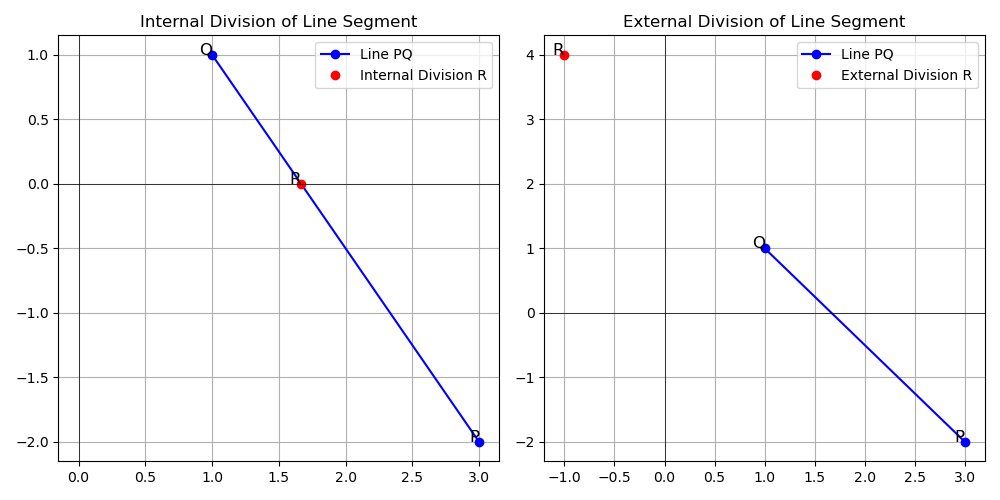
\includegraphics[width=0.8\textwidth]{figs/fig.png}
		\caption{Internal and External division by point R}
	\end{figure}   
\end{frame}

\end{document}